\documentclass[11pt,a4paper,fleqn]{article}

\usepackage[ansinew]{inputenc}
\usepackage[mathscr]{eucal}
\usepackage{amsmath,amssymb,amsthm}
\usepackage{graphicx}
\usepackage{caption}
\usepackage{subcaption}
\usepackage{hyperref}
\usepackage{gensymb}
\usepackage{listings}
\usepackage{float}

\allowdisplaybreaks
\flushbottom

\setlength{\textwidth}{160.0mm}
\setlength{\textheight}{245.0mm}
\setlength{\oddsidemargin}{0mm}
\setlength{\evensidemargin}{0mm}
\setlength{\topmargin}{-15mm} %{-20mm} for arXiv, {-15mm} for printing on A4
\setlength{\parindent}{5.0mm}

\hypersetup{colorlinks, linkcolor=blue, citecolor=blue, urlcolor=blue}


\makeatletter
\long\def\@makecaption#1#2{%
  \vskip\abovecaptionskip\footnotesize
  \sbox\@tempboxa{#1. #2}%
  \ifdim \wd\@tempboxa >\hsize
    #1. #2\par
  \else
    \global \@minipagefalse
    \hb@xt@\hsize{\hfil\box\@tempboxa\hfil}%
  \fi
  \vskip\belowcaptionskip}
\makeatother

\marginparwidth=17mm \marginparsep=1mm \marginparpush=4mm

\newtheorem{theorem}{Theorem}
\newtheorem{lemma}{Lemma}
\newtheorem{corollary}{Corollary}
\newtheorem{proposition}{Proposition}
{\theoremstyle{definition}
\newtheorem{definition}{Definition}
\newtheorem{example}{Example}
\newtheorem{remark}{Remark}
\newtheorem*{remark*}{Remark}
}


\begin{document}

\par\noindent {\LARGE\bf
Using Deep Learning to Predict Future Climate
\par}

\vspace{6mm}\par\noindent{\bf

}


\vspace{6mm}\par\noindent
Author: Chelsea Beaton \par\noindent
E-mail: ctbeaton@mun.ca


\vspace{9mm}\par\noindent\hspace*{8mm}\parbox{140mm}{\small\looseness=-1
Climate change has been very prevalent in society for many years now, and for good reason. The Earth has been changing rapidly in recent years, with temperatures rising and more extreme weather conditions occurring more often, and accurately predicting how the Earth is changing is becoming very important. This is a key step in preventing or possibly reversing the effects of climate change. There are many ways in which this has been done through the years, but a relatively new method of predicting climate is done by deep learning. User friendly programs like NeuralProphet are making deep learning more accessible, which means it is now being used in many more ways than when it was first created.
}\par\vspace{5mm}


Keywords:
Climate change,
Deep learning


\section{Introduction}

Deep learning can be defined as a type of machine learning based on artificial neural networks in which multiple layers of processing are used to extract progressively higher level features from data. Deep learning allows computers to learn from experience and understand the world in terms of a hierarchy of concepts, with each concept defined through its relation to simpler concepts.\cite{Goodfellow-et-al-2016} Based on this definition, it can be hard to imagine what this type of learning would be used for. In reality, deep learning has been used in a multitude of different ways, such as providing the tools necessary to create self-driving cars, intelligent assistants, medical image analysis \cite{ker2017deep}, climate prediction, etc. \par
When first diving into the topic of deep learning, it can seem like a very heavy and inaccessible topic. A lot of the ideas thrown out are abstract and hard to understand. However, like most things do, deep learning is becoming more and more accessible over time. For example, programs like NeuralProphet let users train neural networks with only a few lines of code. Neural prophet is a python library for modelling time-series data based on neural networks. This means that data can be used to train a program to predict future data. With deep learning becoming more user friendly, more and more people will be able to learn and utilize deep learning in an increasing number of ways. \par
One of the uses of deep learning mentioned before is climate prediction. If there is a set of data containing information about the climate in a certain area for a period of time, a neural network can be trained to predict the climate in that area for future years. In doing so, the similarities and differences between the predicted climate and the actual climate in the future can be analyzed. This is a great way to represent climate change, as it visualizes the differences between what the climate `should have' been and what it actually is.

\section{Methods}\label{sec:Methods}
The first thing needed is a set of data to work with. The data used in this report contains the average daily temperature (in \textdegree F) of 157 U.S. and 167 international cities.\cite{daytonwebsite} This data gives the Region, Country, State (if applicable), City, Date and AvgTemperature (the daily average temperature in that city). Within the data set there are `missing values' - dates in which there was no available data - that are recorded as -99. It is important to get rid of these values because they would throw off the graphs if left in. To do this, a dataframe is set to: 
$$df = df[df.AvgTemperature != -99]$$
This saves all of the entries except for the ones with a value of -99. \par
Our data needs to be in SI units, so to change the values from Fahrenheit to Celsius, the AvgTemperature column is set to 
$$AvgTemperature = \frac{AvgTemperature - 32}{1.8}$$
Now, the data for individual cities can be prepared to be used to create graphs for that specific city. To do this, a new data frame is defined to contain the dates and average temperatures for that unique city. In order to make sure the predicted climate for that city is accurate, the first 80\% of the data will be used to train the NeuralProphet model and the last 20\% is used to compare the actual temperature of the city to the predicted temperature. To do so, the data is split:
$$data80, data20 = m.split\_df(data, valid\_p=0.2)$$
Finally, a future data frame is created using Neural Prophet. The length of this data frame should be the same as the last 20\% of our original data frame so that the two graphs will begin and end at the same point. Plotting these two data frames on the same graph allows the predicted temperatures from Neural Prophet to be compared to the actual temperatures of the city. This will show how accurate the Neural Prophet predictions were. 

\section{Results}\label{sec:Results}
The first graph observed is for Fairbanks, Alaska. As seen from the graph, the actual temperatures of Fairbanks follow the same pattern as the predicted temperatures. However surprisingly, it can be seen that as the years go on, Fairbanks is experiencing much colder than average temperatures. Although the average yearly temperature is rising, more extreme temperatures in the winter are occurring more often. Climate change does not just mean that the Earth is getting warmer, it can also mean more extreme weather in general.\cite{palmer2014record} This can easily be seen from the graph in Figure 1(a). 

\begin{figure}[h]
     \centering
     \begin{subfigure}[b]{0.4\textwidth}
         \centering
         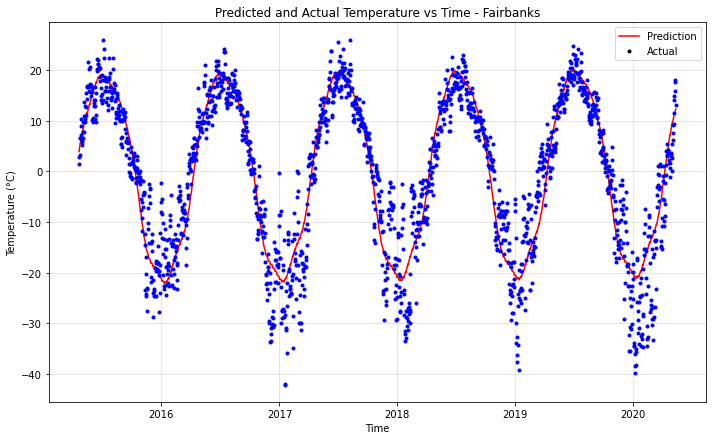
\includegraphics[width=\textwidth]{Fairbanks.png}
         \caption{Predicted and average temperature vs. time in Fairbanks.}
     \end{subfigure}
     \hfill
     \begin{subfigure}[b]{0.5\textwidth}
         \centering
         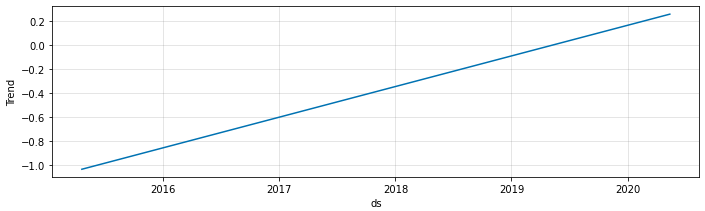
\includegraphics[width=\textwidth]{FairbanksComponents.png}
         \caption{Average yearly temperature vs. time in Fairbanks.}
     \end{subfigure}
     \caption{Graphical analysis of temperatures in Fairbanks, Alaska.}
\end{figure}

The next city looked at is for Cairo, Egypt. As seen from the graphs below, the actual temperatures in Cairo follow the same pattern as the predicted temperatures. Although there are some hotter and colder outliers, the overall pattern is very similar. When looking at the average yearly temperature graph something interesting can be seen. The average yearly temperature is decreasing. Because of climate change and global warming, it would be expected to see a rise in average yearly temperatures in all cities, but climate change does not affect every area equally.\cite{forbeswebsite} There are many factors that influence climate, and in areas where climate change is not having much influence, there could be a drop in average yearly temperature, as can be seen from Figure 2(b).

\begin{figure}[h]
     \centering
     \begin{subfigure}[b]{0.4\textwidth}
         \centering
         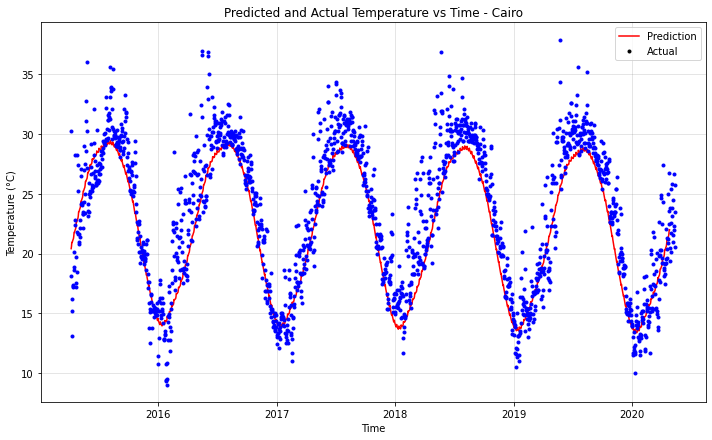
\includegraphics[width=\textwidth]{Cairo.png}
         \caption{Predicted and average temperature vs. time in Cairo.}
     \end{subfigure}
     \hfill
     \begin{subfigure}[b]{0.5\textwidth}
         \centering
         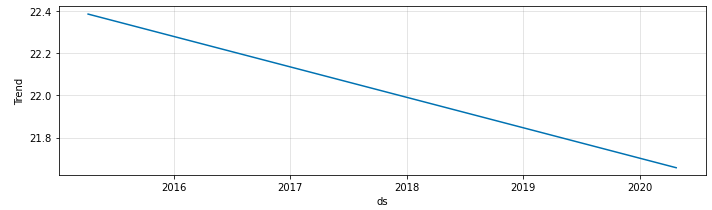
\includegraphics[width=\textwidth]{CairoComponents.png}
         \caption{Average yearly temperature vs. time in Cairo.}
     \end{subfigure}
     \caption{Graphical analysis of temperatures in Cairo, Egypt.}
\end{figure}

Next, the predicted and actual temperatures for Singapore are observed. Although the hottest temperatures are not much higher than the average temperature (the highest recorded temperature was around 32\textdegree C when the average temperature was around 29\textdegree C), as can be seen from Figure 3, hotter than average temperatures are occurring more often.


\begin{figure}[h]
    \centering
    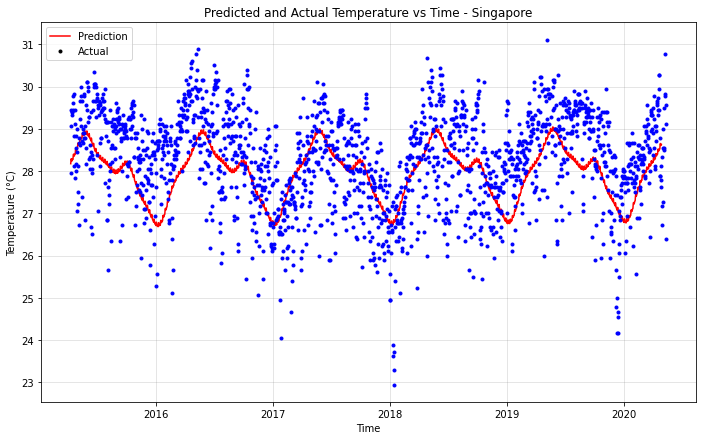
\includegraphics[width=0.4\textwidth]{Singapore.png}
    \caption{\label{fig:graph}Predicted and average temperature vs. time in Singapore.}
\end{figure}

The last graph observed is for Los Angeles, California. Like previous graphs shown, Los Angeles' predicted temperatures and actual temperatures seem to follow a similar pattern. Some years have more hotter than average days, but it seems from the graph that they are having more colder than average days in the past few years. The coldest day recorded on the graph was around 5\textdegree C when the average temperature for that time was around 15\textdegree C. The hottest day was around 30\textdegree C when the average temperature for that time was around 20\textdegree C.

\begin{figure}[h]
    \centering
    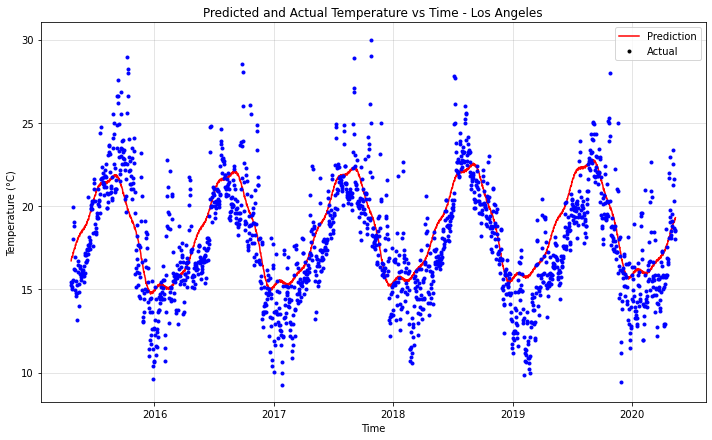
\includegraphics[width=0.4\textwidth]{Los Angeles.png}
    \caption{\label{fig:graph}Predicted and average temperature vs. time in Los Angeles.}
\end{figure}

\section{Conclusion}\label{sec:Conclusion}
In summary, the effects of climate change can be represented in many ways. Currently, there are advancements being made to predict and possibly prevent climate change and deep learning is one of those advancements. Although the method used in this paper was not 100\% accurate in predicting what the future climate in these cities were, it was a good way to represent global warming because it visualized a comparison between what the temperature `should have' been and what it actually was. \par
Although this was a helpful tool in visualizing the effects of climate change, one downside is in order to see if the predictions were accurate, real life data is needed to compare it to. If predictions are created for the future, there will not be a way to tell if they are accurate until time passes. This data was able to be analyzed right away because the program utilized data from the past. Overall, this method of visualizing climate change was helpful even though it had its disadvantages.

\section{Appendix}\label{sec:Appendix}
After reading in the climate data frame and converting the temperatures to \textdegree C, the following code was used to train the NeuralProphet time series prediction model:

\begin{lstlisting}
#Creating the "City" dataframe
la = df[df[`City'] == "Los Angeles"]
la[`Date'] = pd.to_datetime(la[`Date'])
data = la[[`Date', `AvgTemperature']]
data.dropna(inplace=True)
data.columns = [`ds', `y']

m = NeuralProphet()

#Taking 80% of the data to use to train the NeuralProphet program
#Taking 20% of the data to compare to our prediction and see 
#if it was accurate 
data80, data20 = m.split_df(data, valid_p=0.2)

m.fit(data80, freq="D", epochs=100)

#Using the 80% of data to predict the climate in the future
future = m.make_future_dataframe(data80, periods=len(data20))

#Plotting the predicted temperature
forecast = m.predict(future)
plot1 = m.plot(forecast)

#Plotting the actual temperature
plt.plot(data20.ds, data20.y,`b.')

\end{lstlisting}

\footnotesize\setlength{\itemsep}{0ex}

\bibliographystyle{abbrv}
\bibliography{cite}

\end{document}
